%% artigo-exemplo.tex

\documentclass[a4paper]{IEEEtran}
\usepackage[utf8]{inputenc}
%\usepackage{latin}
\markboth{}{}
\usepackage[portuges]{babel}

\usepackage{algorithm}
\usepackage{algpseudocode}
\ifCLASSINFOpdf
  \usepackage[pdftex]{graphicx}  
\else
  \usepackage[dvips]{graphicx}
\fi

\graphicspath{{}} 

\renewcommand{\footnoterule}{\noindent\rule{0.5\columnwidth}{0.5pt}\vspace*{3pt}}

\begin{document}

% Título (usar \\ para quebra de linha)
\title{API design and implementation of a management interface for SDN whitebox switches}

% author names and affiliations
% use a multiple column layout for up to three different
% affiliations
\author{\IEEEauthorblockN{Rubens Jesus Alves Figueiredo $^$}%
%\thanks{r.figueiredo.52@gmail.com}
\IEEEauthorblockN{Dr. Ana Cristina Costa Aguiar $^$}%
%\thanks{$^\dag$Contacto orientador}
\IEEEauthorblockN{Dr. Hagen Woesner$^$}%
%\thanks{$^\ddag$Contacto co-orientador}
}
% make the title area
\maketitle

% \markboth{Uma parte}{Outra parte}

\begin{abstract}
The rising requirements of today's cloud services require the evolution of networking infrastructure to support the increasing amount of data that is processed
every day. This means that data center network operators must design or adapt their cloud networking environments to provide a stable and reliable connection.
Better optimized infrastructure often also means cost reductions in network utilization and energy savings.

\par As networks grow larger and more complex, systems must be put in place that allow for closely monitoring the resources that make up the network, while also 
allowing for a certain freedom for the possible constant change of the network. As such, typical vendor solutions don't really fit into this ever changing landscape,
since they present very solid and vertically integrated solutions. The Software Defined Networking paradigm, however, is able to solve this issue, since it enables
the centralized control of the underlying networks, providing visibility and control over the network's devices, simplifying error diagnosis and troubleshooting. 

\par In this work we propose a modular management system for cloud data center Software Defined Networking controllers, providing system administrators a simple
platform to view their network's topology, monitor networking devices ports, etc. The modularity also provides a simple platform to extend the functionality 
of the networking controllers, that can be used to implement detection of network abnormalities and optimize flow forwarding paths, among others.
\end{abstract}

\begin{IEEEkeywords}
Software-Defined Networking, Cloud Data centers, OpenFlow, Networks, SDN
\end{IEEEkeywords}

\section{Introduction}

\IEEEPARstart{T}{he} rapid expansion of the cloud computing environment in the previous decade is related to the increasing demand in computational power that 
applications like distributed databases or data analysis have. Public cloud solutions like Amazon's Web Services, Microsoft's Azure, or private solutions offered
through OpenStack provide a very large pool of resources for developers to deploy applications with ease. Through economies of scale, these vendors have
centralized their solutions in very large scale data centers, consolidating their operations in a single location, allowing increased performance of applications, and
easier maintenance. The offer of virtualisation solutions also contributes to the recent surge in popularity of these systems, due to the less spending in
operational costs and improved utilization of hardware \cite{sims_david_carousels_2011}. Subscription based systems are typically available for renting, allowing 
users to use services on a Virtual Machine.

\par Using open source applications and whitebox hardware has also contributed to the success of these environments, due to the possible cost reductions. Software
Defined Networking (SDN), has proven to be a reliable environment to manage data center environments, due to the centralization of the network
controllers, improved programmability of the network's data plane, and improved management systems. Network programmability, despite not being exclusive to the 
SDN framework, eliminates the effort in individually configuring every network device, which in large scale environments becomes an impossible task. This model
also provides the network engineers and software developers a high level network abstraction that is used to monitor network utilization and optimize resource
utilization.

\par Due to data center's traffic profile, one common challenge for optimizing the networks resource utilization
is the asymmetry of traffic, where most of the networking flows are short-lived, latency-sensitive quick bursts of packets, but do not amount for the total traffic 
in the network. The main contributor for the total traffic volume are the large and long-lived flows, usually called elephant flows. By maintaining a system that
monitors and alarms network operators of the occurrences of large data streams, this will provide insight to the network operators to plan ahead their network 
resources.

\par This document is organized in:

\begin{itemize}
    \item \textbf{Related Work} is an overview of Software-Defined Networking, providing an insight on the protocol behind these environments,
and presenting information on the existing applications. This section also sums up a formal framework for change detection mechanisms;
    \item \textbf{Proposed Architecture} details the proposed architecture for this work, and the technologies used for implementation;
    \item \textbf{Implementation} details the employed technologies
    \item \textbf{Results} provides an overview of the results, by displaying the developed Graphical User Interface, and the results of the change detection method
        implemented for monitoring elephant flows;
    \item \textbf{Conclusion} sums up the main contributions of this work.
\end{itemize}

\section{Related Work}

\section{Proposed Architecture}

\begin{figure}
    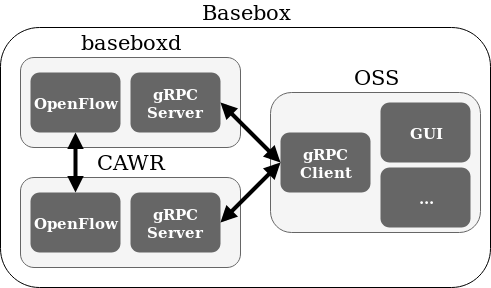
\includegraphics[scale=0.4]{../doc/figures/bisdn/prp_system_low_level.png}
    \caption{Proposed system}
    \label{fig:fig}
\end{figure}

\par We build an Operations Support System (OSS) that provides the basis for the development of applications that monitor the state of the network, using an
implemented API to obtain the relevant information. This system allows further separation of roles in the network, in contrast to a system where the controller would
gather the roles of managing and monitor the network’s status, increasing the load on the controllers. Furthermore, this architecture increases the modularity of 
the components, enabling hot-swapping different modules, and allows parallel development of different features in the monitoring and management stack.

We provide a proof-of-concept composed of two components: the first is a Graphical User Interface (GUI) providing an user friendly interface to display topology and
statistics, and the second is an intelligent system enabling the detection of elephant flows. In this section we describe in a high level way the approaches for the 
development of this system.

\section{Implementation}

We have developed an Operations Support System (OSS), visible in figure \ref{fig:fig}. The controllers had to be extended to support the gRPC interfaces, and this 
connection is accessible through port 5000 on baseboxd and port 5001 on CAWR.  To demonstrate the interfaces capability of exposing the topology and statistics 
information, we have developed a simple Graphical User Interface (GUI) as a proof-of-concept of this platform. This GUI can be accessed via a web page, since this
provides an ease of access to the system. The web page was developed on top of the Django Framework, since it is a framework developed in the Python programming 
language, support for official gRPC integration and ease of implementation. For drawing the topology we used the JavaScript library D3.js.

\section{Results}

\subsection{Graphical User Interface}

The connection between both controllers to the GUI provides the view for both controllers, which means that CAWR will present the view for the physical switches, 
bonded ports and hosts, while the baseboxd only shows the giant switch created by CAWR. Analysis of the global view of the state of the
network, include the addition of displaying configured VLANs in each port, and even provide a way to configure these VLANS via a GUI. Interaction with the nodes is 
possible, and clicking on each provides an insight to the statistics related to the ports in that node.

\subsection{Elephant Flow Monitoring}

\begin{algorithm}[H]
    \caption{Elephant Detection Algorithm - High Level} \label{alg:high_level}
    \begin{algorithmic}[1]
        \Procedure {Elephant Flow Detection}{}
            \State Initialization
            \State Query controller
            \Loop
                \State Calculate prediction error
                \State Predict next values
                \State Detection
                \If {Detection}
                    \State Raise Alarm
                \EndIf
                \State wait 2 seconds
            \EndLoop
        \EndProcedure
       \end{algorithmic}
\end{algorithm}

\par The initialization step of the algorithm is a crucial step for obtaining correct results in the algorithm. These steps, allowing the correct initialization of
the model parameters, including the trend component, and to provide a baseline for the expected traffic on the network. It is assumed that no traffic abnormalities
exist during this stage, but a longer period for initialization can account for short bursts of higher traffic.

\par Time series analysis can generate forecasts for future values, assuming the temporal behaviour is maintained for future observations. During the design phase 
of the algorithm, we selected the exponential smoothing technique, since this is a commonly used technique in the reviewed literature \cite{jasek_usage_2013, 
munz_traffic_2010}, and provides a generally simple way to generate forecasts based in historical data.

\par One of the analysed change detection methods is the CUSUM algorithm. This method is used for monitoring parameters of a sample, by monitoring deviations of the
observations according to a certain target value. Typical implementations of this algorithm are based in an offline approach, calculating the alarm times
with knowledge of the entire data set. The adaptation of the CUSUM algorithm for utilization as an online technique is based on a sliding window that
is updated with every new sample. Applying this method has the advantages of using the CUSUM algorithm without needing extensive changes, while also reducing the 
amount of memory needed to apply this method.

\section{Conclusion}
% referências
\par The main objective for this thesis was building a management system that would integrate with a pre-existing Software-Defined Network controller, exposing 
information for network operators to manage and configure their networking infrastructure. We have built a management environment that extends the previously 
existing system, allowing further developments in the field of Traffic Engineering in the Basebox environment. Complementing this system, we have also designed a
Graphical User Interface for interaction with the users, allowing for simple visualisation of the network’s physical topology, and the display of interfaces’ 
statistics, like the packets and bytes received and sent, or the number of errors.

\par We have also proposed an algorithm that allows for monitoring traffic changes in ports, in order to detect elephant flows in the network. Despite not having 
used the Basebox system for testing this algorithm, due to differences in the testing environment, we believe that the same algorithm can be used for large flow 
detection in the Basebox stack. We have shown that a simple method can be employed by operators to monitor the state of their network, and rely on this algorithm to
provide them with alarms of port changes.

\bibliographystyle{IEEEtran}
%\bibliography{../doc/thesis_reference}

\end{document}
